% -----------------------------------------------
% Template for ISMIR 2010
% (based on earlier ISMIR templates)
% -----------------------------------------------

\documentclass{article}
\usepackage{ismir2012,amsmath,cite}
\usepackage{graphicx}

% Title.
% ------
\title{AMA LAB2: MELODIC TRANSCRIPTION}

% Single address
% To use with only one author or several with the same address
% ---------------
%\oneauthor
% {Names should be omitted for double-blind reviewing}
% {Affiliations should be omitted for double-blind reviewing}

% Two addresses
% --------------
\twoauthors
  {Jakue L\'{o}pez Armend\'{a}riz} {Universitat Pompeu Fabra \\ Music Technology Gorup}
  {H\`{e}ctor Parra Rodr\'{i}guez} {Universitat Pompeu Fabra \\ Music Technology Group}

% Three addresses
% --------------
%\threeauthors
%  {First author} {Affiliation1 \\ {\tt author1@ismir.edu}}
%  {Second author} {\bf Retain these fake authors in\\\bf submission to preserve the formatting}
%  {Third author} {Affiliation3 \\ {\tt author3@ismir.edu}}

% Four addresses
% --------------
%\fourauthors
%  {First author} {Affiliation1 \\ {\tt author1@ismir.edu}}
%  {Second author}{Affiliation2 \\ {\tt author2@ismir.edu}}
%  {Third author} {Affiliation3 \\ {\tt author3@ismir.edu}}
%  {Fourth author} {Affiliation4 \\ {\tt author4@ismir.edu}}

\begin{document}
%
\maketitle
%
\begin{abstract}
A simple melodic transcription method for monophonic phrases is presented.
The fundamental frequency and energy variations are computed to accomplish such task.
First, both methods are individually studied to find their strong and weak characteristics.
Finally, a mixing method for both strategies is proposed. This mixing method is able
to balance the weight of each strategy in order to improve the results for each
analyzed phrase.
\end{abstract}
%
\section{Fundamental Frequency}\label{sec:f0}

The fundamental frequency ${f0}$ of a periodic signal is the inverse of its period, which may be defined as the smallest positive member of the infinite set of time shifts that leave the signal invariant. This definition applies only to \textit{perfectly} periodic signals. However, music or speech are not perfectly periodic, and this is why ${f0}$ estimation becomes a challenge in this field. The concept of subjective \textit{pitch} of a sound usually depends on its fundamental frequency. Over a wide range, they are related in a one-to-one relation. Thus, in this document we will often use the pitch term to refer to the fundamental frequency. In many cases, ${f0}$ estimation algorithms are also often referred as \textit{pitch detection algorithms}.

\subsection{Extraction}\label{subsec:f0_extraction}

We have tested six different ${f0}$ estimation algorithms: Yin, Spectral Comb, Schmitt, Fast Harmonic Comb, Yin with FFT and MELODIA\footnote{http://www.mtg.upf.edu/technologies/melodia}. The First five are included in the aubio\footnote{http://aubio.org/} library. 
After testing all of them with five different melodies, the ones that perform best appear to be Fast Harmonic Comb, MELODIA and Yin. However, MELODIA has a limitation of a maximum frequency of 1760 Hz and it is not giving values for higher frequencies. Comparing Yin and Fast Harmonic Comb algorithms, this last one has shown more accurate estimations and is the one we have chosen for this task (see \figref{fig:yinvsfhc}).

\begin{figure}
 \centerline{\framebox{
 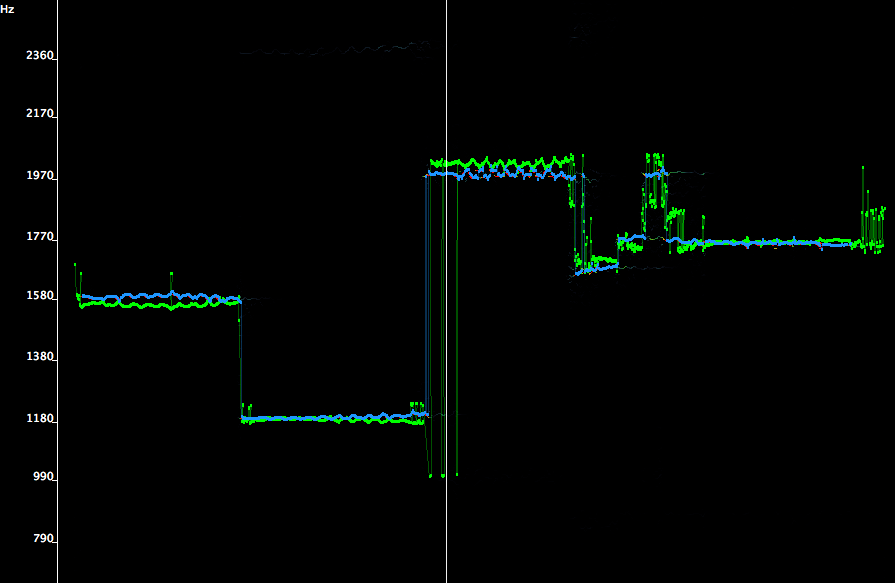
\includegraphics[width=\columnwidth]{figures/FHC-Orange-vs-Yin-Green.png}}}
 \caption{Yin (green), Fast Harmonic Comb (blue) and Spectral peaks (red).}
 \label{fig:yinvsfhc}
\end{figure}

\subsection{Postprocessing}\label{subsec:f0_postpro}
In order to obtain a proper decision function for the transcription some post processing is applied to the output signal of the Fast Harmonic Comb algorithm. 

\subsubsection{Smoothing}
As the algorithm doesn't provide a perfect estimation for every frame, the first step is to smooth the estimation signal. A median filter over 15 frames has been computed (see \figref{fig:f0smooth}). With this smoothing, frames with unexpected values like octave errors and wrong estimations are fixed. The ${f0}$ estimation signal becomes more stable.

\subsubsection{Derivation}
In order to track frequency variations, the fundamental frequency derivative is computed. The output function will have peaks in the frames where there is a change in the ${f0}$ values.

\begin{figure}
 \centerline{\framebox{
 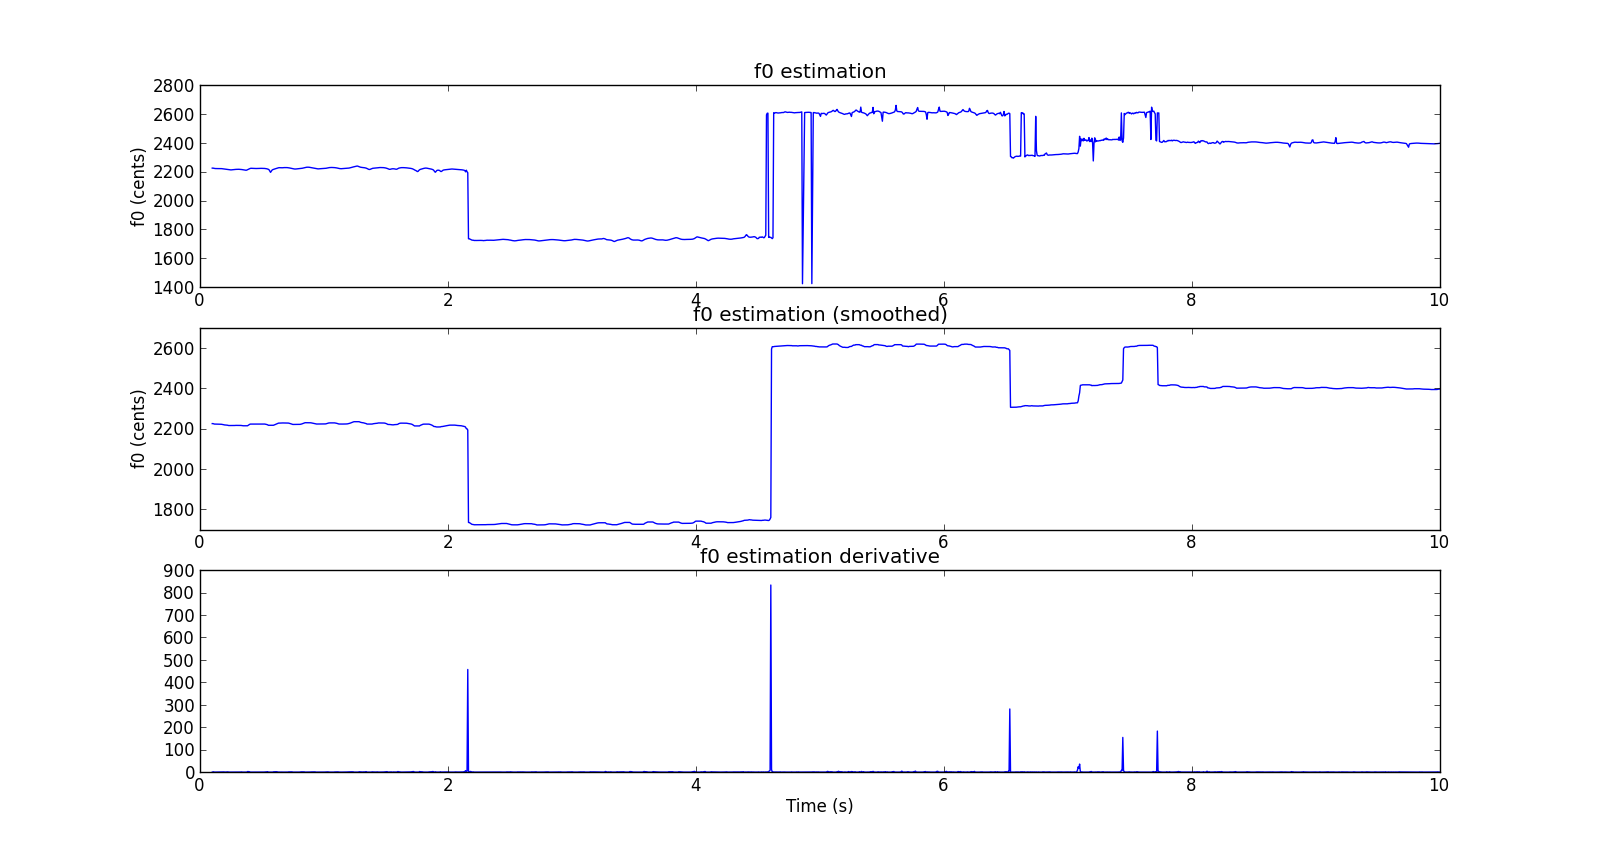
\includegraphics[width=\columnwidth]{figures/f0-vs-f0-smooth.png}}}
 \caption{original f0 estimation (top), smoothed (middle) and derivation (bottom) functions.}
 \label{fig:f0smooth}
\end{figure}

\subsubsection{Peak detection}
To detect the exact position of these changes a peak detection of this derivation function is computed. As we are interested in any kind of pitch change (an increase or decrease in frequency) the absolute value of the function is obtained in advance. At this stage we already had a decision function.
We will check for local maximum that will provide us the exact frame where a frequency change happens.

\section{Energy}
In this section the strategy of using the wave energy for note segmentation is evaluated.

\subsection{Extraction}
The energy strategy tries to take advantage of the fact that when a new note is played there is an increase
in loudness for most instruments. To extract the amplitude of a sound (later converted to loudness) we can use different descriptors:

\begin{itemize}
	\item Energy:
		\begin{equation}
		energy(m) = \frac{1}{N}\sum_{n=-N/2}^{N/2}((x(n+mh))^2w(n)
		\end{equation}	
	\item Root Mean Square (RMS):
		\begin{equation}
		rms(m) = \sqrt{ \frac{1}{N}\sum_{n=-N/2}^{N/2}((x(n+mh))^2 w(n) }
		\end{equation}
	\item Wave envelope:		
		\begin{equation}
		env(m) = \frac{1}{N}\sum_{n=-N/2}^{N/2}|(x(n+mh)|w(n)
		\end{equation}		
\end{itemize}

Usually ${energy}$ is used to obtain the waveform amplitude.
We run several tests changing the descriptor and found no significant difference in our results.
In fact, if we see this descriptors as a function applied to the waveform values (see \figref{fig:energy_descriptors})
the energy is lowering the middle values.
As there is no reason to do such a thing we chose the simplest (and computationally cheapest) descriptor: ${wave\ envelope}$.
Despite of that, in this document we will refer to the result obtained here as ${energy}$.

\begin{figure}
 \centerline{\framebox{
 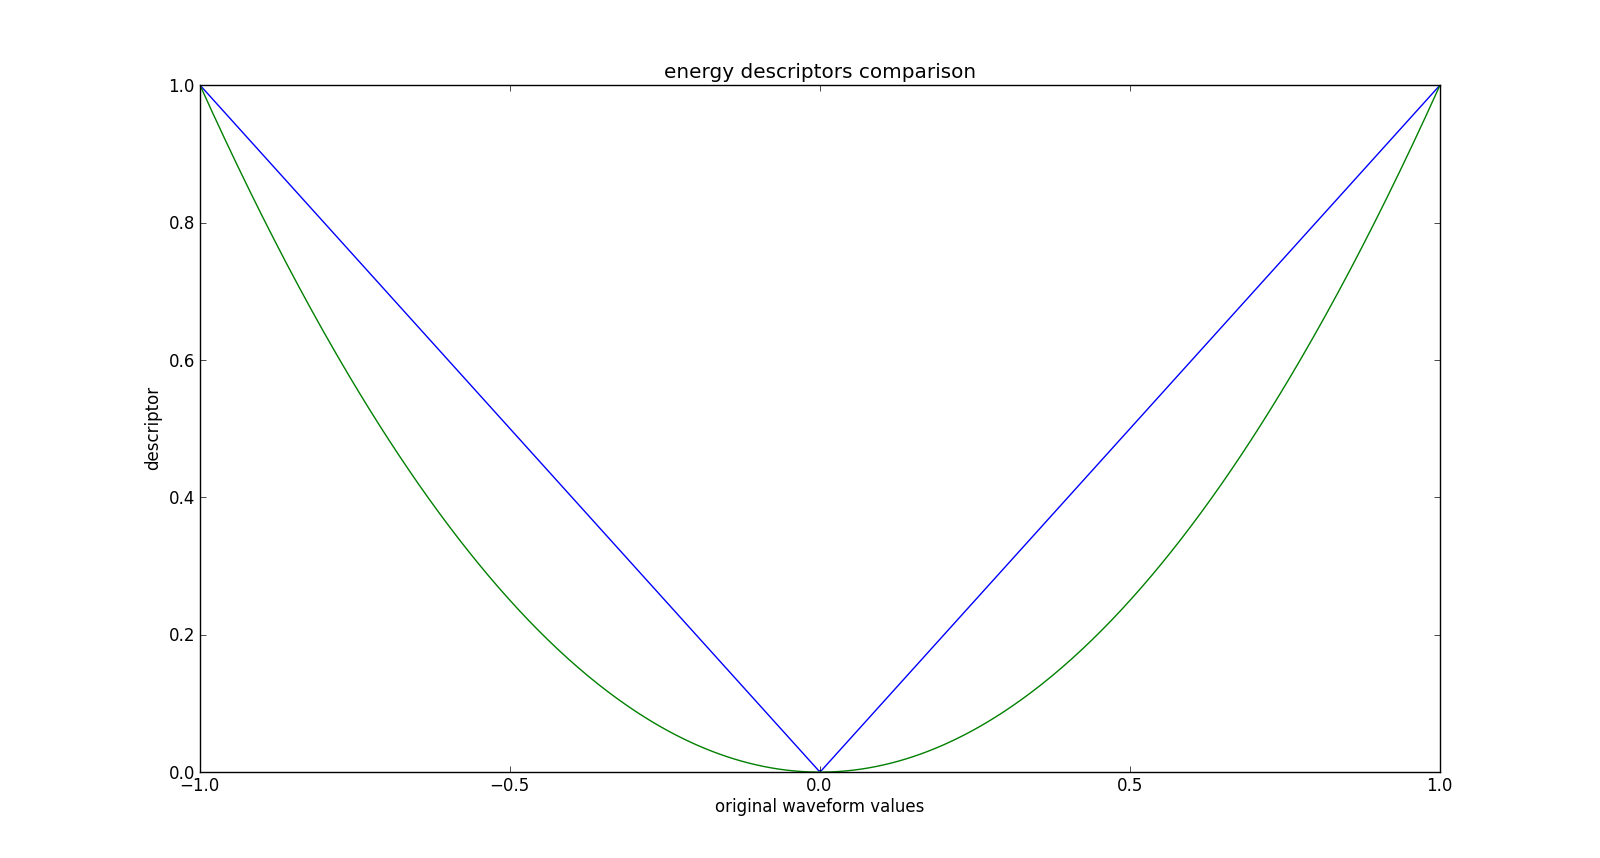
\includegraphics[width=\columnwidth]{figures/energy_descriptors.png}}}
 \caption{Energy descriptors' functions. Blue line: waveform envelope and RMS. Red line: energy. X axis represents the original waveform values
 (with range [-1,1]) and y axis the transformation that descriptors produce. This is a simplistic case with window size = 1.}
 \label{fig:energy_descriptors}
\end{figure} 

\subsection{Postprocessing}
Once we have ${energy}$ computed we need to manipulate it in order to detect were variations occur.

\subsubsection{Loudness}
To make our system detect variations similarly to humans we transformed logarithmically ${energy}$ (this is an approximation of our perception).
It is interesting to point out that this function transforms values in an opposite fashion (not exactly opposed) than the energy descriptor
(${power\ 2}$ function), thus another reason to peak waveform envelope instead.

\subsubsection{Smoothing and derivation}
${Energy}$ is a descriptor that already uses a mean filter and, thus, smooths.
The next step was to compute the derivative (remember we want variations), but this produced a fast changing signal that needed to be re-smoothed.
At first, we tried with another mean filter, but we finally found that the best results were obtained through differentiation with windows.
This consists on computing the difference of the average of two windows (left and right) at each side of current sample.
In all cases we found that a good window size was 25ms (half of the onset tolerance used later in section \ref{sec:eval})

\subsubsection{Peak detection}\label{subsec:energy_peaks}
At this stage we already had the decision function.
A local maximum means an increase in loudness and corresponds to an onset and
a local minimum means a decrease in loudness and corresponds to an offset.
For detecting those peaks we decided to use a different approach (than the one used in fundamental frequency);
instead of searching for any local maximum we only took the greatest maximum given a window size (in our case a 100ms window).
This solved two problems: first, high frequency changes that might still remain after smoothing can produce lots of local small peaks
in larger lobes, and second, this larger lobes can appear too close even though they represent a single onset/offset.

\subsubsection{Tempo matching}
Finally, we tested a post-processing approach based on onsets regularity.
Assuming that the waveform has a constant tempo, we can deduce the beats per minutes (BPM) from onsets' positions 
and discard those onsets that are too far from a simple integer multiple or divisor of BPM.
We implemented a simple algorithm of that idea were we compute the sum of the distance of each onset with its two closest neighbors,
and then we discard those onsets whose value is far away from the mean.
We can see in \figref{fig:energy_bpm} how this method just removes the only remaining incorrect onset and offset.
Despite of that, the implementation was too simplistic and did not behave good enough for other melodies.

\begin{figure}
 \centerline{\framebox{
 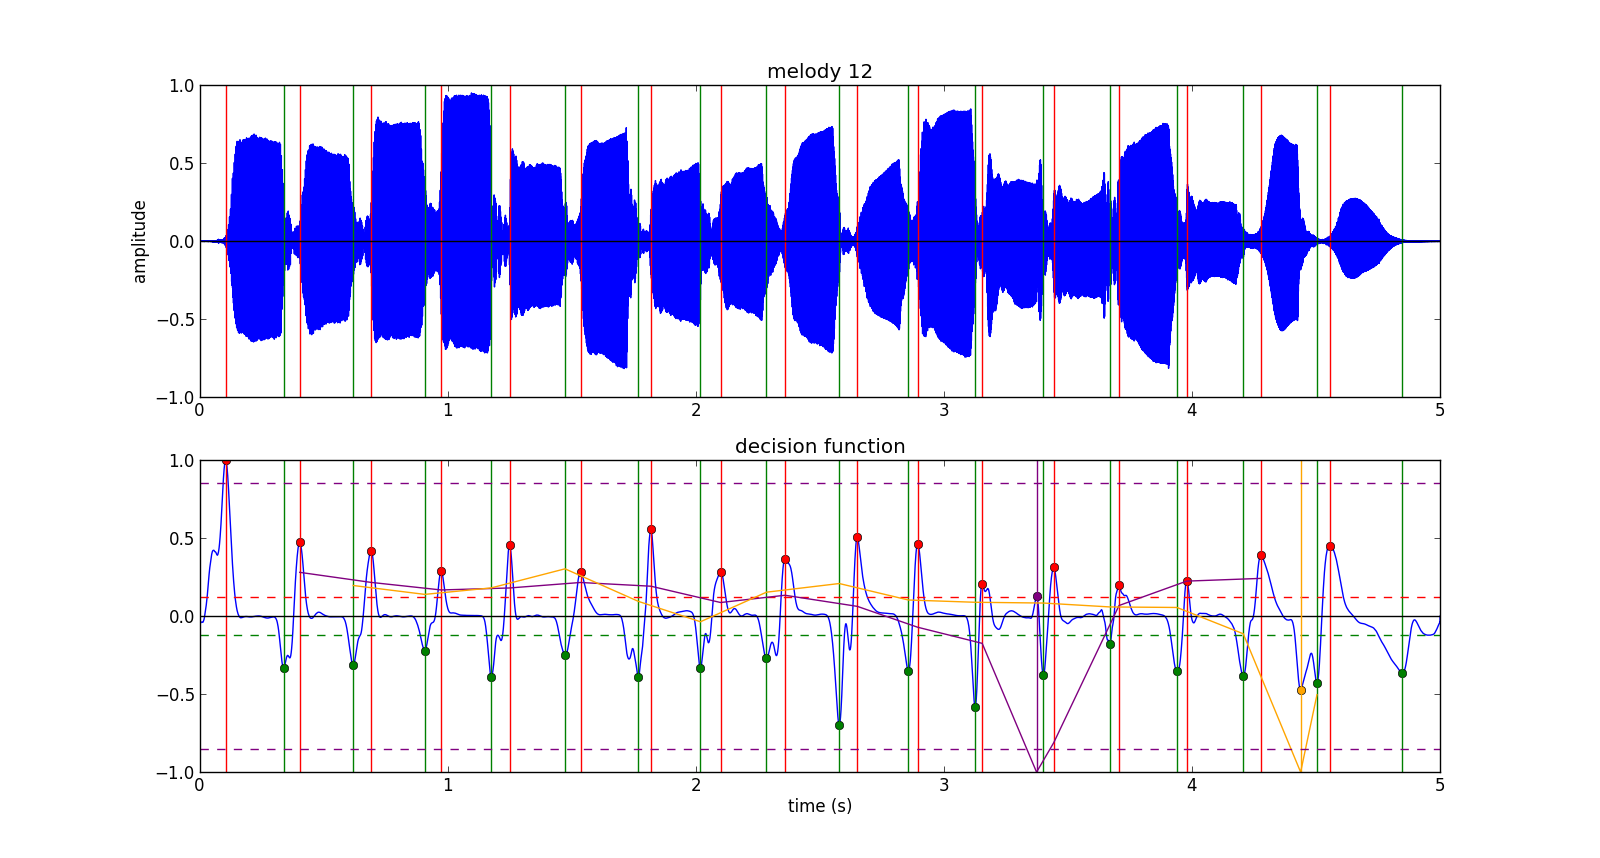
\includegraphics[width=\columnwidth]{figures/energy_bpm.png}}}
 \caption{Energy peak detection with tempo matching. Red: onsets, green: offsets, purple: onset tempo function, orange: offset tempo function}
 \label{fig:energy_bpm}
\end{figure}

\section{Merging decision functions}

In order to obtain a more robust decision function we will implement a function that merges the ones obtained from the pitch and energy descriptors. The sum of both decision functions has appeared to be the most significative approach to merge them. We will first normalize both functions in order to balance them afterwards. This way, coincident peaks are enhanced and lower possible false peaks only contained by one function are lowered. 
For the implementation, a linear interpolation of the ${f0}$ decision function has been computed. This function provides a value for each frame, while the one for the energy does it for each sample. We also had to take into account that the Fast Harmonic Comb algorithm does not provide an output for all the frames, but just for the voiced ones. In case where an unvoiced frame it gives no output and jumps to the next voiced one. Thus, we had to add zeros in those unvoiced frames before the interpolation.

Every instrument and every phrase have their own requirements for the transcription. For example, it will be more convenient to transcribe a piano from the energy decision function (percussive onsets) than from the pitch. In contrast, due to the strong energy variations (tremolo), a flute will be easier to transcribe by taking the pitch. This is why, in our implementation, a mix coefficient to balance the sum of both decision functions can be specified. This parameter will assign a weight to each of the decision functions (see \figref{fig:mixcoef})

\begin{figure}
 \centerline{\framebox{
 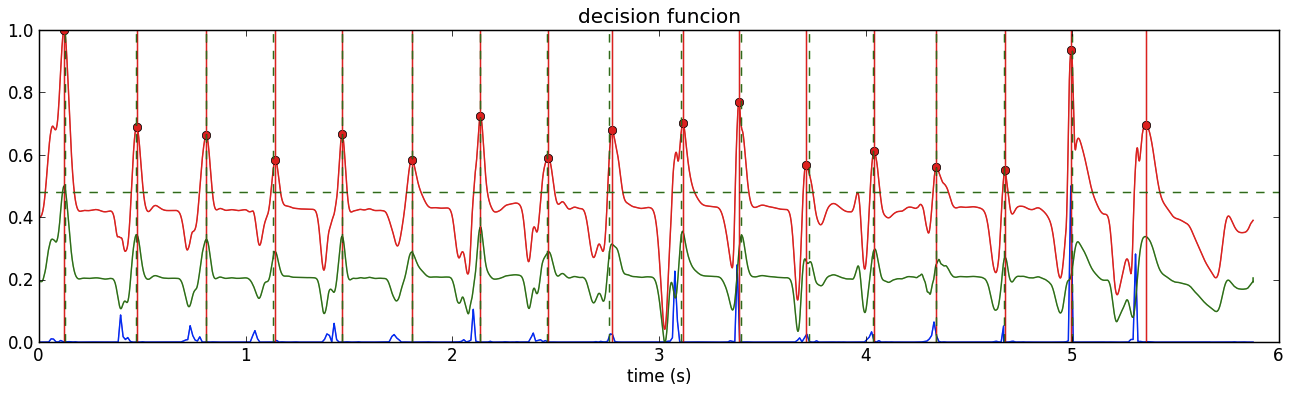
\includegraphics[width=\columnwidth]{figures/mergefx.png}}}
 \caption{Decision functions: Merged (red), f0 estimation (blue) and energy (green). Peak detection: Threshold value (black-dotted horizontal), peaks (red dots), annotated onsets (red lines) and ground-truth (black-dotted vertical).}
 \label{fig:mixcoef}
\end{figure} 

\subsection{Postprocessing}\label{subsec:mix_postpro}

As a first postprocessing step, we will smooth the decision function. This way, double peaks for the same variations that are close in time, but not exactly in the same position, are avoided. We have used a mean filter over a 25 ms. sliding window to compute this smoothing. 

For locating the peaks, we will use the same peak detection algorithm implemented for the energy (see subsection \ref{subsec:energy_peaks})
Due to this, we do not need to care about the presence of double peaks, this function already solves this problem.

\section{Evaluation}\label{sec:eval}

For evaluating the performance of our system we used the method proposed in
MIREX 2012 Audio Onset Detection\footnote{http://www.music-ir.org/mirex/wiki/2012:Audio\_Onset\_Detection}.
This evaluation checks that every ground truth onset has a corresponding detected onset in a range of 50ms.
We did not check the frequency of the notes as we used a 3rd party frequency detection algorithm.
The final evaluation is done through the f-measure formula also proposed in MIREX.

\subsection{Results}\label{subsec:results}

For obtaining the results we have selected 5 melodies from the database provided. The melodies are \textit{'melody4'} (Flute), \textit{'melody12'} (Oboe), \textit{'melody18'} (Piano playing \textit{sustained}), \textit{'melody19'} (Piano playing \textit{fast}) and \textit{'melody23'} (Strings). The reasons to choose this melodies are the presence of different instruments and that we have access to the annotated files\footnote{Annotations provided by E. G\'omez}. This annotated files will be considered to be the ground-truth for our tests.
 
First, for each phrase, we will specify the mix coefficient for obtaining the merge function. For the flute phrase (\textit{'melody4'}) the energy decision function is too unstable. For this reason, the mix coefficient is set so that only the pitch decision function is taken. In contrast, for the piano playing sustained (\textit{'melody18'}), both pitch and energy decision functions are stable, but the energy one provides a more clear solution. In this case, the mixing coefficient has been set to 60 \% of energy function and 40 \% of pitch function. The weights are equally balanced for all the rest of them, that is, 50\% of each decision function.

As a first approach, once the merged decision function is defined, we have manually selected the threshold for each of the melodies in order to obtain the best possible results. For this case, we obtain a precision of 0.95, recall f 0.91 and a 0.92 f-measure values averaged over all melodies (see \tabref{tab:manualfmeasure})

\begin{table}
 \begin{center}
 \begin{tabular}{|l|c|c|c|c|c|c|c|}
  \hline
  melody		&	4		&	12		&	18		&	19		&	23		&	mean			\\
  \hline
  precision	&	1.00		&	0.94		&	1.00		&	1.00		&	0.79 	&	0.95			\\
  recall 	&	0.86		&	1.00		&	0.76		&	0.98		&	0.92 	&	0.91			\\
  f-measure	&	0.92		&	0.97		&	0.88		&	0.99		&	0.85 	&	\textbf{0.92}	\\  
  \hline
 \end{tabular}
\end{center}
 \caption{Precision, recall and f-measure for each evaluated melody using manually annotated threshold and mixcoef.}
 \label{tab:manualfmeasure}
\end{table}

As a second approach, we have tried to automatize the process by setting up an automatic threshold value. By looking at the values of the manually selected thresholds, we have tried to relate them to any parameter that can be extracted directly from the merged decision function. We have observed that the mean of this function appears to be not very far away from the optimal threshold. For this reason, we have performed a grid search by multiplying the mean by a factor (from 0.9 to 1.25). \tabref{tab:autofmeasure} shows that the best recall is obtained for 0.9 and 0.95 multiplier factors, the best precision is obtained for 1.25 and the best balance between both, that is, the best f-measure is obtained for 1.15. We can see how by setting up the automatic threshold the performance of our algorithm decreases from an f-measure of 0.92 to 0.78.

\section{Conclusions}

\subsection{Fundamental frequency (Jakue)}

We can observe how fundamental frequency or pitch variations can allow us to perform note segmentation in some cases. 
Even though the implementation or evaluation of the pitch estimation algorithm was not our goal neither our task, we have to take into account that it is still an unsolved problem. The Fast Harmonic Comb pitch estimation algorithm performs correctly but not perfectly. 
For this reason, in order to minimize the unexpected values of the estimator the smoothing step has to be taken. 

The decision function obtained from fundamental frequency variations appears to be specially useful for sounds with fixed-pitch instruments or for any instrument when notes are played in a non-arpeggiated way. When the transition between notes is clear, for example, the flute in \textit{'melody4'} has a very unstable energy, but clear pitch variations that allow a proper segmentation.

However, for arpeggiated notes or when notes overlap due to reverberation effects, the pitch estimation algorithm approach we have used fails. For this case a polyphonic approach may be taken into account. In the case when big vibratos appear, the decision function can appear to be too noisy. We may not be able to determine if the frequency change is just over the same note (vibrato) or it is already a new one. 

\subsection{Energy (Hector)}

Experiments analyzed in this report confirm our inital theory that stated that amplitude variations are useful to perform note segmentation.
We analyzed three descriptors to measure the amplitude envelope: energy, root mean square, and waveform envelope.
Even though the descriptor that is usually used is energy we observed it transforms the original signal reducing middle valued amplitudes,
producing a undesired deformation.
In opposite, RMS and waveform envelope behave more linearly, thus we finally chose the waveform envelope descriptor because it is
the cheapest to compute of both.

Next, we realized that making our system respond to amplitude in a similar way to human loudness perception, i.e. logarithmically, produced bette results.
Moreover, as a waveform can rapidly vary we needed to get rid of high frequency components to make loudness variations appear uniform and stable lobes.
For that purpose we derivated with a two windows mean difference and used local window peak detection.

Energy, as a method for note segmentation, is useful for those sounds with a strong and quick attack (e.g piano)
but performs poorly when it is not present (e.g. flute).
As this method is based on loudness variation, stable sounds are required and, thus, signals presenting strong tremolos are not very suitable for it.
From another point of view, this method can approximately perform as good as we are able to visually distinguish notes from a graphic representation of the waveform.
It is also interesting to point out that the energy method, as opposite to the frequency method, is not also able to detect notes onsets
but also offsets; an extra information that could be used for further post-processing and improvement.
Eventually, it is important to distinguish which instruments or sounds are suitable for this method before using it.

\subsection{Final (together)}

In this lab we have approached the problem of melody transcription from and audio source. 
This involves two main problems: extracting the pitch and segmenting the notes.

First, in order to obtain pitch we evaluated different fundamental frequency estimation methods, mainly based on autocorrelation and spectral analysis.
Even though we finally chose Fast Harmonic Comb, our decision was based on its better overall performance for our small set of examples.
Currently, there is no method that performs better for all cases and, because of that, it is always crucial to consider which audio material
will be analyzed to use the most suitable method.

Second, we studied note segmentation using two different methods: fundamental frequency variations and energy variations.
Both methods have its weak and strong points but, what is more important, they are different.
This fact allowed us to merge them in a way that, first, segmentation was more reliable when both coincided,
and second, we could balance the decision impact of every method based on the kind of source that was analyzed.

The problem of melody transcription is not a well defined problem.
This means that even us cannot agree on how to do it manually. 
We have experimented that by ourselves when we have faced some ground truths that we would have annotated differently.
Despite of that, our main conclusion is that there is no general approach for melody transcription.
Choosing proper methods for every source is a crucial element.
For that reason, we think that our proposed merging strategy plays a main role on improving the results.
Furthermore, we believe that introducing new descriptors would be the next obvious step.
Finally, a strategy for automatically balancing each descriptor in the merging function would led to a more general solution.

\begin{table}
 \begin{center}
 \begin{tabular}{|l|c|c|c|c|c|c|c|c|}
  \hline
  th. mul	&	0.9				&	0.95				&	1.0		&	1.05		&	1.1		&	1.15				&	1.2		&	1.25 \\
  \hline
  prec.		&	0.30				&	0.47				&	0.53		&	0.70		&	0.76		&	0.81				&	0.82		&	\textbf{0.83} \\
  recall 	&	\textbf{0.95}	&	\textbf{0.95}	&	0.94		&	0.93		&	0.88		&	0.83				&	0.79		&	0.75 \\
  f-meas.	&	0.57				&	0.58				&	0.64		&	0.76		&	0.77 	&	\textbf{0.78}	&	0.77		&	0.75 \\  
  \hline
 \end{tabular}
\end{center}
 \caption{Precision, recall and f-measure mean of the five melodies.
 Each column is computed for a different threshold result of a value (th. mul) that multiplies the mean of the decision function}
 \label{tab:autofmeasure}
\end{table}

\section{Appendix}

The implemented code can be found here: *******

%\section{Footnote}
%
%Indicate footnotes with a number in the text.\footnote{This is a footnote.}
%Use 8pt type for footnotes. Place the footnotes at the bottom of the page on which they appear.
%Precede the footnote with a 0.5pt horizontal rule.
%
%\subsection{Figures, Tables and Captions}
%
%All artwork must be centered, neat, clean, and legible.
%All lines should be very dark for purposes of reproduction and art work should not be hand-drawn.
%The proceedings are not in color, and therefore all figures must make sense in black-and-white form.
%Figure and table numbers and captions always appear below the figure.
%Leave 1 line space between the figure or table and the caption.
%Each figure or table is numbered consecutively. Captions should be Times 10pt.
%Place tables/figures in text as close to the reference as possible.
%References to tables and figures should be capitalized, for example:
%see \figref{fig:example} and \tabref{tab:example}.
%Figures and tables may extend across both columns to a maximum width of 17.2cm.
%
%\begin{table}
% \begin{center}
% \begin{tabular}{|l|l|}
%  \hline
%  String value & Numeric value \\
%  \hline
%  Hello ISMIR  & 2012 \\
%  \hline
% \end{tabular}
%\end{center}
% \caption{Table captions should be placed below the table.}
% \label{tab:example}
%\end{table}
%
%\begin{figure}
% \centerline{\framebox{
% \includegraphics[width=\columnwidth]{figure.png}}}
% \caption{Figure captions should be placed below the figure.}
% \label{fig:example}
%\end{figure}
%
%\section{Equations}
%
%Equations should be placed on separated lines and numbered.
%The number should be on the right side, in parentheses.
%
%\begin{equation}
%E=mc^{2}
%\end{equation}
%
%\section{Citations}
%
%All bibliographical references should be listed at the end,
%inside a section named ``REFERENCES,'' numbered and in alphabetical order.
%Also, all references listed should be cited in the text.
%When referring to a document, type the numbering square brackets
%\cite{Author:00} or \cite{Author:00,Someone:10,Someone:04}.
%
%\begin{thebibliography}{citations}
%
%\bibitem {Author:00}
%E. Author:
%``The Title of the Conference Paper,''
%{\it Proceedings of the International Symposium
%on Music Information Retrieval}, pp.~000--111, 2000.
%
%\bibitem{Someone:10}
%A. Someone, B. Someone, and C. Someone:
%``The Title of the Journal Paper,''
%{\it Journal of New Music Research},
%Vol.~A, No.~B, pp.~111--222, 2010.
%
%\bibitem{Someone:04} X. Someone and Y. Someone: {\it Title of the Book},
%    Editorial Acme, Porto, 2012.
%
%\end{thebibliography}

%\bibliography{ismir2012template}

\end{document}
